\chapter{Project management}

\section{Risk management}

\begin{table}[!htb]
  \centering
  \begin{tabular}{|p{0.16\columnwidth}|c|c|p{0.42\columnwidth}|}
  \hline
  \textbf{Risk (event)} & \textbf{Likelihood} & \textbf{Impact} & \textbf{Action} \\ \hline
  Camera module failure & Low & High & Buy redundant camera modules. \\ \hline
  Jetson board failure & Low & High & Find another one, or find alternative ways to continue the project. \\ \hline
  Test facilities not available & Low & Medium & Check in advance. \\ \hline
  ECS file storage server is slow & Medium & Medium & Use my own laptop. \\ \hline
  Supervisor is away at meeting & High & Low & Read literatures, continue implementations. \\ \hline
  Unexpected accident or illness & Low & High & Try to avoid. Have multiple backups. \\ \hline
  Unable to implement camera driver & Medium & High & Find easy alternatives, or read frames from video files. \\ \hline
  Unable to implement some algorithms & Medium & High & Find easy alternatives. \\ \hline
  \end{tabular}
  \caption{Risk assessment}
  \label{man:risk}
\end{table}

\subsection{Board failure}

During the second semester, the Jetson board accidentally failed on 3rd, Match. I was probing a current sensor resistor on the board, then unintentionally short circuited the 12V power rail to the 3.3V power rail. Although the CPU, GPU cores and some peripheral interfaces survived, two of the power rails were still in short circuit condition and cannot be easily diagnosed. As a result, USB, Ethernet and HDMI interfaces were not functioning. The board can only be controlled through a UART interface, with a voltage level converter chip. Power consumption analysis would also be affected by the two short circuited power rails.

I quickly transferred the algorithm development to a general purpose computer to continue working on it. This could be done only because all the source codes were regularly backed up on the git server. Having recognised that the board is only essential for power consumption modelling, reasonable results were still possible even without the board. The algorithms can run on a general computer, most analyses are still possible. Finally, after some negotiation with my supervisor, another board was available for use, the development was then transferred to the new board.

\section{Time management}

The topic of project changed once during week 7 in semester 1. The previous topic (\aref{Appendix:brief_prev}) was about reducing power consumption for algorithms that are utilising General Purpose GPU (GPGPU) technique, by adaptively controlling calculation precision. The NVIDIA Jetson TK1 development platform was decided to be used in this project. However, after investigated into the topic and experimented with some algorithms, the purposed precision control did not contribute significant impact on computation quality. Not much power saving would be possible to be made.

Therefore, I decided to change the project topic. The current project topic (\aref{Appendix:brief}) was quickly determined. The same hardware platform was still used, so that the time invested in the previous project was not wasted. Therefore, I was able to quickly catch up with the progress.

The Gantt chart was also changed due to project topic changing, as shown in \fref{gantt_prev} and \fref{gantt_rev}. The time invested for previous project topic was treated as background reading. \fref{gantt} shows the actual time spend on each of the items.

\begin{figure}[H]
  \centering
  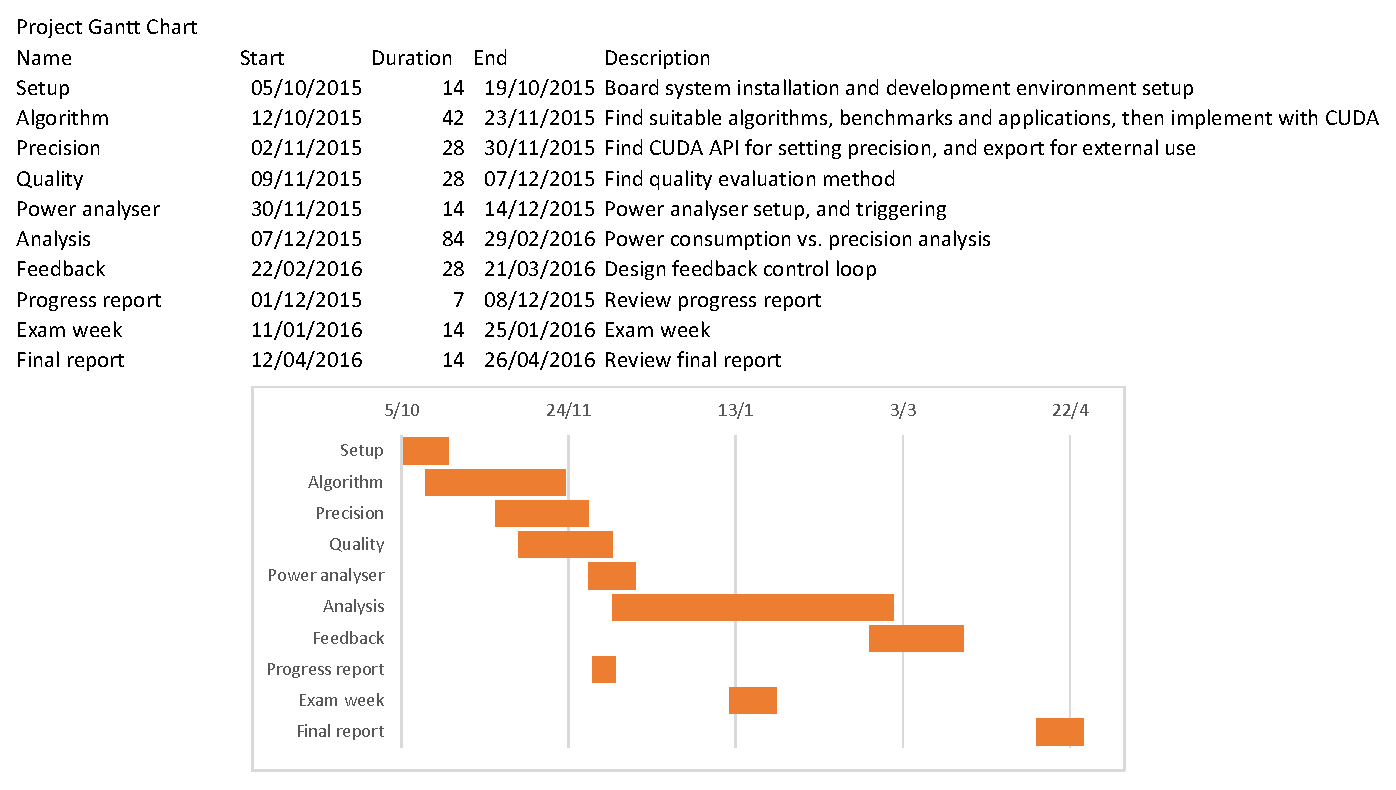
\includegraphics[width=\columnwidth]{Gantt_previous}
  \caption{Previous Gantt chart}
  \label{gantt_prev}
\end{figure}

\begin{figure}[H]
  \centering
  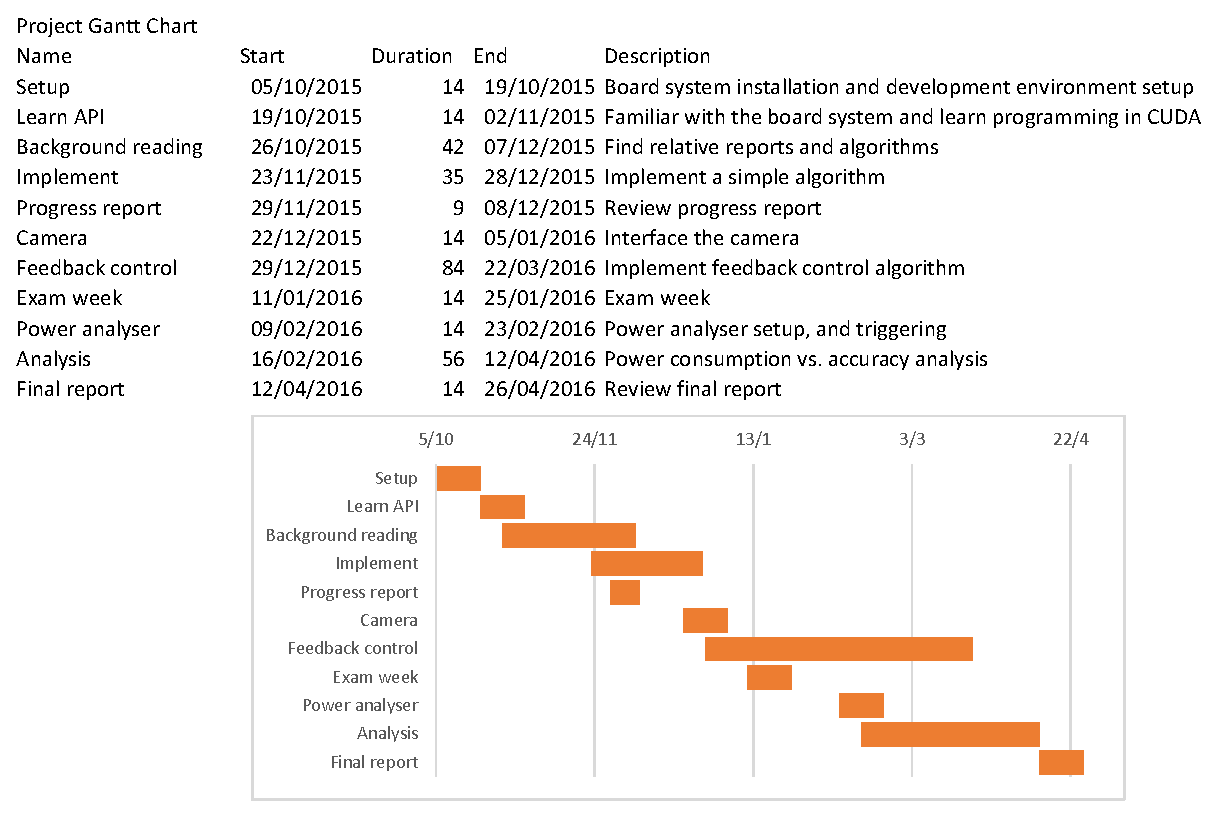
\includegraphics[width=\columnwidth]{Gantt_interim}
  \caption{Revised Gantt chart}
  \label{gantt_rev}
\end{figure}

\begin{figure}[H]
  \centering
  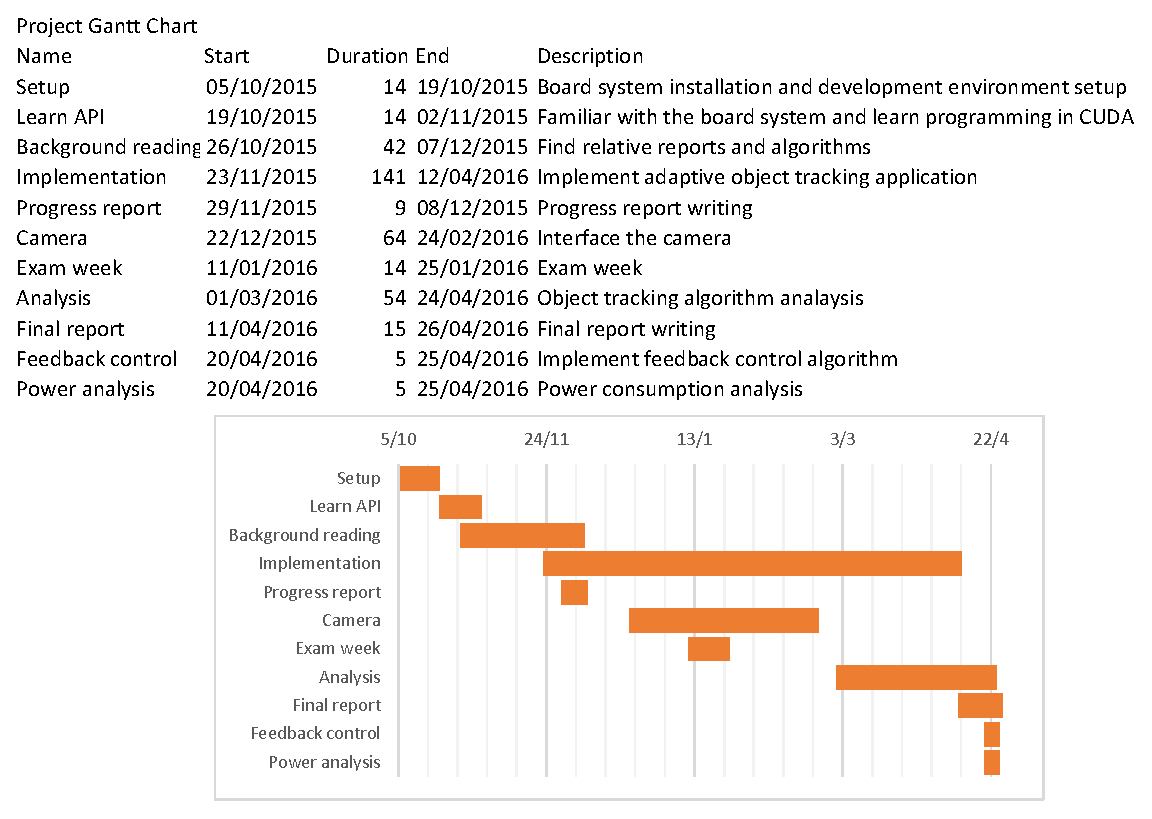
\includegraphics[width=\columnwidth]{Gantt}
  \caption{Actual time usage}
  \label{gantt}
\end{figure}

\section{Backing up}

%Source code management.
%Documents and materials.

The git version control system \cite{git} was used in this project. It has the feature that allows multiple users collaborate on the same repository. However, this is an individual project, git was used purely for backing up source code version history and synchronisation between multiple devices. Well-known git hosting website GitHub \cite{github} and university's SourceKettle server \cite{sourcekettle} were used for multiple backups.

All documents, background literals and materials used by the project were backed up using Microsoft's OneDrive service.

%\section{Remaining work}

%\begin{itemize}
%  \item Movement tracking based on blob detection (Section \ref{bg:tracking}, \ref{impl:tracking}).
%  \item A camera module need to be ordered and interfaced.
%  \item Automatic frame rate reduction based on tracking result.
%  \item Hardware downsampling and cropping based on ROI.
%  \item If time allows, energy-efficient object recognition may be implemented.
%\end{itemize}
